%
% The first command in your LaTeX source must be the \documentclass command.
\documentclass[sigconf]{acmart}

\settopmatter{printacmref=false}
\renewcommand\footnotetextcopyrightpermission[1]{} % removes footnote with conference information in first column
\pagestyle{plain} % removes running headers

%
% defining the \BibTeX command - from Oren Patashnik's original BibTeX documentation.
\def\BibTeX{{\rm B\kern-.05em{\sc i\kern-.025em b}\kern-.08emT\kern-.1667em\lower.7ex\hbox{E}\kern-.125emX}}
    
% Rights management information.
% This information is sent to you when you complete the rights form.
% These commands have SAMPLE values in them; it is your responsibility as an author to replace
% the commands and values with those provided to you when you complete the rights form.
%

\settopmatter{printacmref=false} % Removes citation information below abstract
\renewcommand\footnotetextcopyrightpermission[1]{}

%
% These commands are for a JOURNAL article.
%\setcopyright{acmcopyright}
%\acmJournal{TOG}
%\acmYear{2018}\acmVolume{37}\acmNumber{4}\acmArticle{111}\acmMonth{8}
%\acmDOI{10.1145/1122445.1122456}

%
% Submission ID. 
% Use this when submitting an article to a sponsored event. You'll receive a unique submission ID from the organizers
% of the event, and this ID should be used as the parameter to this command.
%\acmSubmissionID{123-A56-BU3}

%
% The majority of ACM publications use numbered citations and references. If you are preparing content for an event
% sponsored by ACM SIGGRAPH, you must use the "author year" style of citations and references. Uncommenting
% the next command will enable that style.
%\citestyle{acmauthoryear}

%
% end of the preamble, start of the body of the document source.
\begin{document}

%
% The "title" command has an optional parameter, allowing the author to define a "short title" to be used in page headers.
\title{Analyzing Matlab's Matrix-Matrix Multiplication for Auto-Optimization}

%
% The "author" command and its associated commands are used to define the authors and their affiliations.
% Of note is the shared affiliation of the first two authors, and the "authornote" and "authornotemark" commands
% used to denote shared contribution to the research.
\author{Kevin Cox}
\email{shkevin@unm.edu}
\orcid{}
\affiliation{%
  \institution{University of New Mexico}
  \streetaddress{1 University of New Mexico}
  \city{Albuquerque}
  \state{New Mexico}
  \postcode{}
}

%
% By default, the full list of authors will be used in the page headers. Often, this list is too long, and will overlap
% other information printed in the page headers. This command allows the author to define a more concise list
% of authors' names for this purpose.
%\renewcommand{\shortauthors}{Trovato and Tobin, et al.}

%
% The abstract is a short summary of the work to be presented in the article.
\begin{abstract}

In recent years, several algorithms have been proposed that lower the asymptotic upper bound of matrix-matrix multiplication. Many of these algorithms are very efficient at taking advantage of caching and cold-miss reductions. The low level differences that make these algorithms so efficient can, and were, implemented in C. These C implementations were then compared against Matlab, a language that boasts the efficiency of their linear algebra operations. Matlab has reported that their built-in matrix-matrix multiplication has been auto-optimized in order to decrease the amount of CPU time and wall time used to calculate the desired result. The experiments performed in this paper have shown that Matlab performs implicit multi-threading at reasonable matrix sizes and appears to out-perform all of these C implementations.

\end{abstract}

%
% A "teaser" image appears between the author and affiliation information and the body 
% of the document, and typically spans the page. 
%\begin{teaserfigure}
%  \includegraphics[width=\textwidth]{sampleteaser}
%  \caption{Seattle Mariners at Spring Training, 2010.}
%  \Description{Enjoying the baseball game from the third-base seats. Ichiro Suzuki preparing to bat.}
%  \label{fig:teaser}
%\end{teaserfigure}

%
% This command processes the author and affiliation and title information and builds
% the first part of the formatted document.
\maketitle

\section{Introduction}

Matrix multiplication of two n x n matrices can be difficult to efficiently write, and is often asymptotically bounded by the cube of the input size n. Until recently, the best algorithm was created by Don Coppersmith and Shmuel Winograd, aptly named the Coppersmith-Winograd algorithm \cite{coppersmith-winograd}. The algorithm is built off the Schonhage-Strassen algorithm and achieves an O($n^{2.375477}$) when multiplying two n x n matrices. The algorithm that marginally trumps the Coppersmith-Winograd algorithm was developed by Stothers, Vassilevska-Williams, and Le-Gall, and achieves an asymptotic upper bound of O($n^{2.3725}$) \cite{gall}. This algorithm furthers the work of the Coppersmith-Winograd algorithm, but is often not used due to hardware limitations.

This paper attempts to answer questions about Matlabs' asymptotic growth for both CPU time and wall time for their built in matrix multiplication. Matlab is purpose made for matrix mathematics and achieves relatively good performance for several mathematical operations. This paper compares eight algorithms implemented in C, in order to answer if Matlab does automatically optimize the matrix-matrix multiplication algorithm based off of input size. Matlabs' optimized multiplication is assumed to automatically determine the best matrix-matrix algorithm, as well as implicitly multi-thread the built in linear algebra operations inherent to matrix multiplication. The Matlab version tested was 9.4.0.813654 (R2018a).

\section{Methods}

When there is an increase in square matrix size n, Matlab automatically optimizes the algorithm used. This hypothesis was tested similar to a repeated measures experiment. The null hypothesis will state that the median values for CPU time will be the same for each algorithm. The alternative hypothesis will state that the CPU times are different based off of matrix size. The factor tested between all algorithms, including the C algorithms, is the size of the square matrix n. The treatment used to test the size factor was performed by running all algorithms with the same size factors. The size factors were randomly shuffled between each algorithm in order to limit the potential nuisance factors or any confounding factors. Each algorithm was timed based off of CPU time and wall time of their respective algorithms. CPU time was output in order to conclude whether caching or any processor operations, such as context switching, was a possible nuisance factor. Wall time was used to provide more insight as to whether caching was was a nuisance factor. If the wall time for the algorithm was statistically similar to the CPU time, then this might imply that the caching effect was minimum for that algorithm.

The algorithms tested were different levels of optimization's for matrix multiplication, where the control was Matlabs' built in matrix multiplication. These optimization's include blocking the matrices in order to optimize caching, looping over matrix dimensions such that the number of cold misses is limited, and vectorizing the matrices. Matlab implicitly vectorizes matrices, in order to linearly transform the matrix into column vectors and then applies the desired operations. A total of nine algorithms were tested, eight of which were written in C, and the one Matlab built in function. All algorithms were tested by iterating over the randomly permuted matrix sizes, applying varying levels of iterations inversely proportional to the matrix size, and then iterating again for the number of experiments. The result is a triply-nested loop. The randomized size iteration is used to reduce variance and limit any potential nuisance factors. The second iteration loop is used as a replicate for each size of the matrix. The inner-most loop is used to increase the number of repeated measures between the experiments. The matrices used in the matrix-matrix multiplication were generated by a uniformly random distribution for each size, effectively giving a unique design point for each size within each algorithm. This distribution was shifted to be between $[-1,1]$ for each algorithm. The performance measure used for all experiments was the CPU time and the wall time of the multiplication contained in the triply-nested loop. Each algorithm was tested on a high-performance computer with one node per algorithm, with each node containing eight cores and 6GB of ram per core. The underlying operating system used was linux, with an Intel Xeon Nehalem EP processor.

The experiment for each algorithm was initially set up with 30 different matrix sizes ranging from $n=31,..,10,000$. For each matrix size, an iteration was performed, where the iteration was from 1 to an inverse proportional number dependant on the matrix size. The same iteration was performed 5 times. This gave a total of $4,142,635$ design points for both CPU time and wall time. Due to the inherent independence between each algorithm, a Wilcoxon rank-sum test (Mann-Whitney U-test) can be calculated to determine if we can reject our hypothesis at the 5 percent significance level.

By comparing CPU time to wall time, Matlabs' implicit multi-threading should be visible. If Matlab implicitly multi-threads their built in matrix multiplication function (*, mtimes), then this will be seen with an increased CPU response time, but a lower wall response time. This suggests that the CPU time will be $np*cputime$, where $np$ is the number of processors. The variation in matrix-matrix multiplication algorithms should be seen with an inconsistency of increasing response time as the size of the matrix increases. This would suggest that the constant modifier for the cubic asymptotic growth varies with size. This may be shown by providing a cubic reference function for all sizes. Each algorithm will be compared against the control, attempting to verify if the underlying distribution and asymptotic complexity is statistically different. 

\section{Results}

\begin{comment}
Present the results of your experiments (use tables, plots, prose, and statistics
as appropriate). State whether the experimental results falsify your hypotheses.
You will be expected to use the statistical tools you were taught in the first half
of the semester.
You should include p-values, confidence intervals, and effect sizes. You may
use whatever plots you believe are most appropriate to communicate your results, but you must also include at least one notched box plot with significance
values clearly marked.
Be careful to only present the quantitative data and discuss how they support
or falsify your hypotheses. This is not the place to include explanations of why
the results are the way they are.
Be careful of statistical pitfalls. For example, if you use a statistical test
that assumes normality you have to justify that assumption.
\end{comment}

Comparing the results of the performed experiment provides insight into the run-time analysis for each algorithm. Each algorithms' performance has been calculated against Matlab as the control. The results of the analysis on the CPU times can be seen in figure \ref{matlab}. The cubic reference line was generated by creating a vector, starting from 1 to the maximum matrix size 10,000, and taking the cube of this vector. It's apparent that the asymptotic growth for Matlab's built in matrix-matrix multiplication is bounded by $O(cn^{3})$, as expected. However, the constant growth term c is much smaller than 1. This holds true for every algorithm that was analyzed, and can be seen in table \ref{tab:speedup}. The growth term was calculated by simply taking the expected value of the largest matrix, then dividing by the cube of the maximum size. The speedup, when compared to Matlab, can be seen alongside the growth term. This speedup was calculated by dividing each algrothms' growth term by Matlabs' growth term. This value gives the expected CPU performance speedup that Matlab has over the C algorithms. The expected value was used for all sizes, due to the invariant nature for each matrix size. The total variance in the entire system, for each size, was minimal. This allowed for any analysis to disregard any additional variance reduction techniques.

\begin{figure}[h]
  \centering
  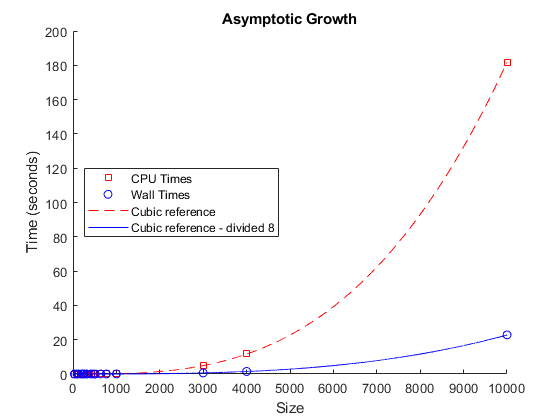
\includegraphics[width=\linewidth]{graphs/matlab.png}
  \caption{This figure shows the asymptotic growth for Matlabs' built in matrix multiplication. The reference lines are cubic, with varying constant growth terms.}
  \Description{}
  \label{matlab}
\end{figure}

\begin{table}
  \caption{Matlab Speedup Over the Algorithms (CPU times)}
  \label{tab:speedup}
  \begin{tabular}{rrr}
    \toprule
    Matlab&Growth Term&Speedup\\
    \midrule
    Matlab   & 1.82e-10 & 1 \\
    Row      & 1.01e-09 & 5.545 \\
    Blas     & 6.81e-09 & 37.49 \\
    Col      & 5.51e-09 & 30.31 \\
    Genvect  & 2.91e-10 & 1.60 \\
    Autovect & 6.37e-10 & 3.51 \\
    Naive    & 2.96e-09 & 16.27 \\
    Copy     & 5.09e-10 & 2.80 \\
    Blocked  & 5.34e-10  & 2.94 \\
  \bottomrule
\end{tabular}
\end{table}

Since there was minimal difference between the wall time and CPU time of each algorithm, the wall time measurement has not been shown. Rather, all Analyses were performed on the CPU time measurement. Due to the large number of design points used for each algorithm, the expected value for each matrix size, for each algorithm, was used to compare against the control. The CPU time comparison between Matlab and the initial eight C algorithms yielded significantly different response times for each. The three best algorithms, including Matlab, can be seen in table \ref{tab:times}. These specific algorithms were chosen to be displayed by calculating the minimum times for the expected values for each size. The chosen algorithms were decided based off of the produced frequency for which algorithms provided the minimum CPU times. It's important to note that the matrix sizes shown in table \ref{tab:times} is a subset of the experimented sizes. These values were chosen to minimize the table size, while displaying various increasing matrix sizes.

\begin{table}
  \caption{Best Algorithms with Various Samples (CPU times)}
  \label{tab:times}
  \begin{tabular}{rrrr}
    \toprule
    Size&Matlab&Copy&Genvect\\
    \midrule
    31    & 1.6e-05     & 0.000024    & 0.000012 \\
    128   & 0.00095     & 0.001       & 0.00053 \\
    255   & 0.005       & 0.0079      & 0.0042 \\
    321   & 0.01        & 0.016       & 0.0081 \\
    512   & 0.03        & 0.063       & 0.032 \\
    769   & 0.102       & 0.22        & 0.11 \\
    1000  & 0.206       & 0.47        & 0.28 \\
    3000  & 4.99        & 12.73       & 7.83 \\
    4000  & 11.83       & 30.09       & 17.66 \\
    10000 & 181.75      & 509.31      & 291.09 \\
  \bottomrule
\end{tabular}
\end{table}

Since normality couldn't be determined between the design points in the data set, a two-tailed Wilcoxon rank-sum test was calculated. The results of the test can be seen in table \ref{tab:wilcoxon}. The test was performed on the subset of data that provided the 3 best algorithms in terms of CPU times. This table shows the p-values associated with using Matlab as the control and comparing against the other 2 C algorithms. The ${95\%}$ confidence interval is shown for median value for that algorithm.

\begin{table}
  \caption{Wilcoxon Rank-Sum Test Summary (CPU times)}
  \label{tab:wilcoxon}
  \begin{tabular}{rrrr}
    \toprule
    Aglorithm&p-value&95\% CI&Conclusion\\
    \midrule
    Copy & 4.43e-193 & [0.12,0.13] & Reject Null Hypothesis\\
    Genvect & 4.19e-12 & [0.06,0.06] & Reject Null Hypothesis\\
    Blocked & 4.67e-193 & [0.14,0.14] & Reject Null Hypothesis\\
  \bottomrule
\end{tabular}
\end{table}

\begin{figure}[b]
  \centering
  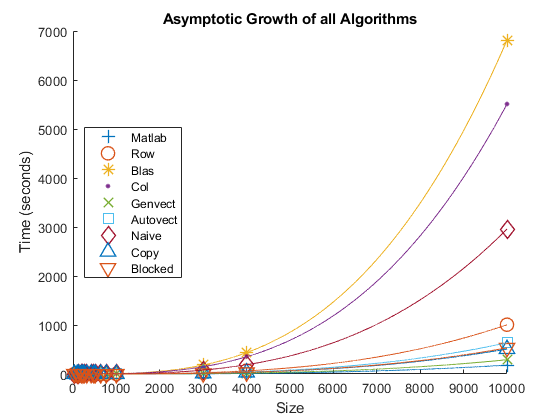
\includegraphics[width=\linewidth]{graphs/all.png}
  \caption{Asymptotic growth for all algorithms. The lines connected each algorithm design point was calculated by the cubic reference, similar to figure \ref{matlab}.}
  \Description{}
  \label{all}
\end{figure}

\section{Discussion}

\begin{comment}

Discuss how the experiments you performed address your questions from the
introduction. Describe plausible causal relationships that explain your results.

\end{comment}

The difference in CPU times and wall times for Matlab shown in figure \ref{matlab} is significant. Wall time is reported based off of how long the matrix-matrix multiplication ran overall. If CPU time is higher than wall time, then this suggests that the number of processors performing the work on the multiplication is greater than one. The experiments were performed on a single node with 8 processors. This scalar value is approximately the amount greater than the CPU time is, compared to the wall time. This can be seen in the figure, where both reference lines have been shown. The invariant nature for Matlabs' response time when increasing the matrix size suggests that the hypothesis that Matlab alters the algorithm used based off of size fails to be shown. This can be concluded by the strictly cubic increase of the response time with each increasing matrix size. However, it does show that Matlab implicitly multi-threads their linear algebra operations in the built in matrix-matrix multiplication. Note that the C functions compared against were not explicitly multi-threaded, and it is unknown whether the algorithms are implicitly multi-threaded. But, comparing the asymptotic growth terms for each algorithm in table \ref{tab:speedup} and figure \ref{all} further supports the claim that Matlab auto-optimizes.

The statistical significance for the algorithms that produced the 3 best CPU times can be seen in table \ref{tab:wilcoxon}. This table was produced by performing additional experiments on the size ranges $480-10,000$. This range was determined to produce the largest differences between the 3 best algorithms. This experiment did additional replications to further determine the variation for each algorithm. The total number of replications used was similarly calculated by the inverse proportion of the size, but with a smaller scaling factor in the denominator. The resulting number of design points were $20x$ greater than the number that was originally used. Table \ref{tab:wilcoxon} shows the p-values for comparing the median values of Matlab to three of the closest algorithms to Matlabs' CPU time. The results indicated that the median values are statistically unequal, therefore we reject the null hypothesis for the algorithms at the $5\%$ Significance level. Although, it was evident that the median values were significantly different just by visually comparing the provided figures. By comparing the 2 best algorithms, Matlab and genvect, further proof has been recorded that these algorithms are statistically different. This can bee seen in figure \ref{boxplot}. Since the notches in the box plot do not overlap, it can be concluded that the true medians do differ. This data reflects the matrix-size $n = 3000$ and was chosen since it reflects the point at which each algorithm CPU times appears to diverge from each other. Matlab claims to use LAPACK, a variant of LINPACK that has incorporated level 1 Basic Linear Algebra Subroutines (BLAS) \cite{matlabMethod}. BLAS was one of the algorithms tested in these experiments. Matlab performed significantly better than this BLAS version and can be seen in figure \ref{all}. This suggests that Matlab does appear to be implicitly multi-threading their linear algebra operations. While the question of whether Matlab auto-optimizes the matrix multiplication algorithm based off of size could not be dis-proven, it does appear that the use of implicit multithreading is inherent to their built-in multiplication.

\begin{figure}[h]
  \centering
  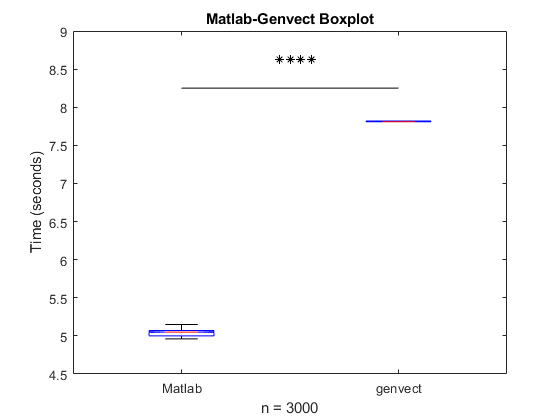
\includegraphics[width=\linewidth]{graphs/boxplot.png}
  \caption{Boxplot of Matlab and genvect. Genvect was the algorithm that produced the closest CPU times. The whiskers show the the 25th and 75th percentile, while the notch shows the medians of the algorithms.}
  \Description{Boxplot for matlab and genvect.}
  \label{boxplot}
\end{figure}

\pagebreak
%
% The next two lines define the bibliography style to be used, and the bibliography file.
\bibliographystyle{ACM-Reference-Format}
\bibliography{sample-base}

\end{document}
